\subsection*{Log ind}
I systemet benyttes en log ind-funktion til at beskytte og identificere den enkelte bruger. Brugeren skal her angive log ind-information, der vil tillade adgang til brugerinformation i form af private oplysninger og tidligere resultater, tilknyttet den givne bruger. Aktiviteterne for log ind fremgår af \autoref{fig:logind}.    

\begin{figure} [H]
\centering
\textbf{Aktivitetsdiagram: Log ind}\par\medskip
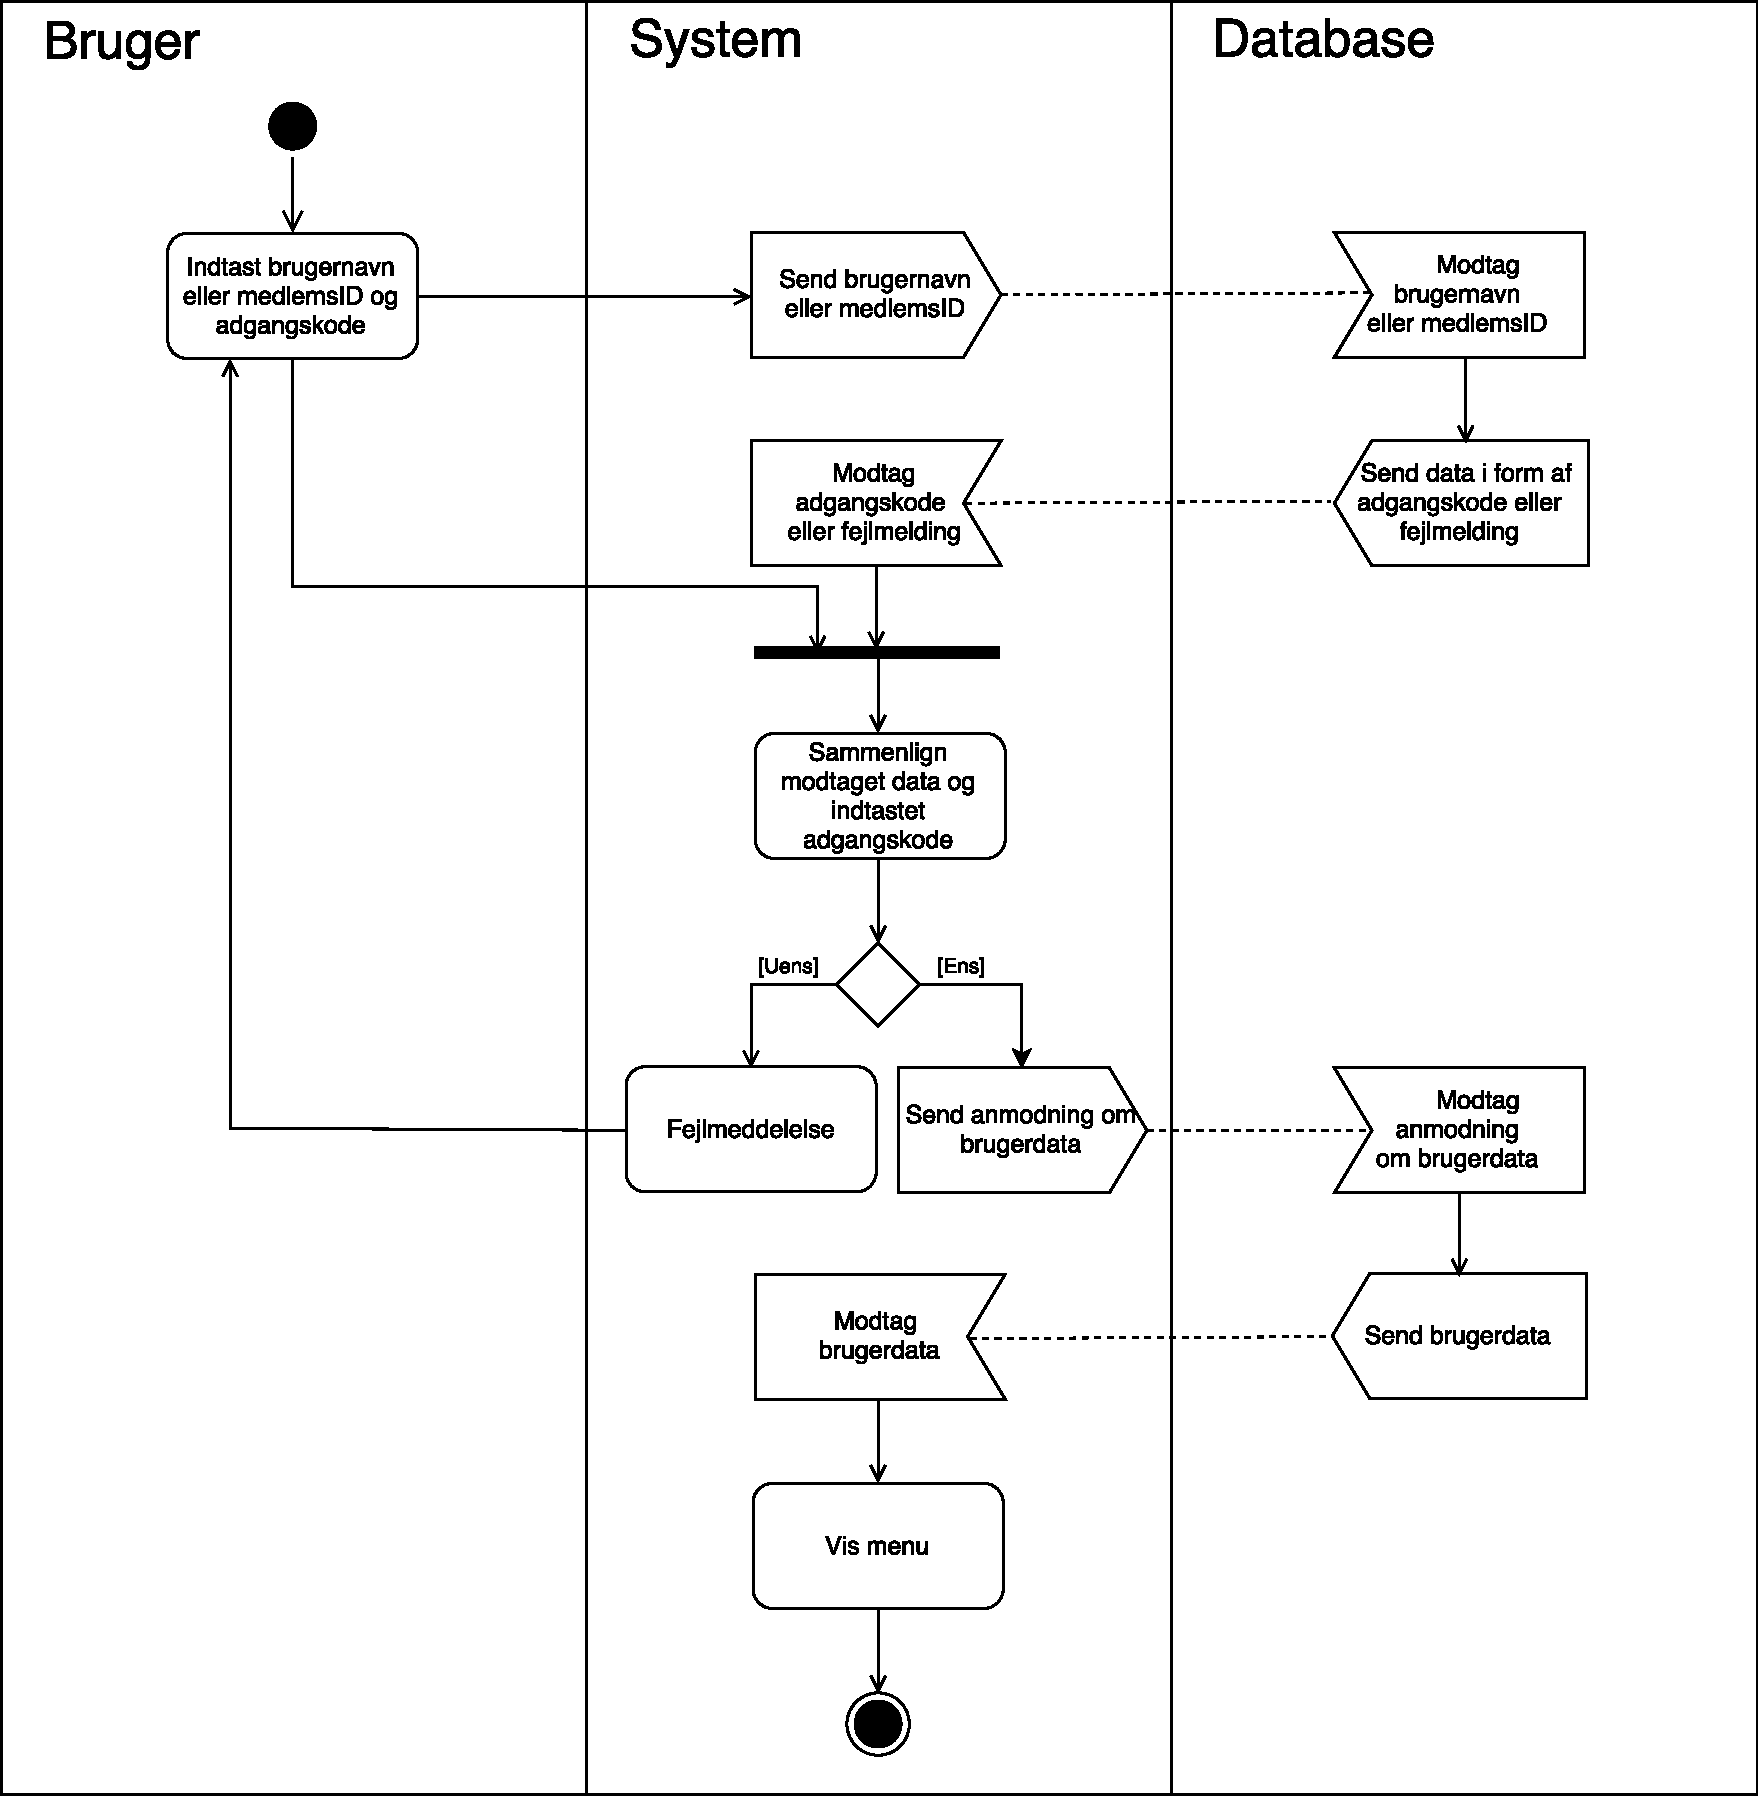
\includegraphics[width=1\textwidth]{figures/aktivitetsdiagram/Logind}
\caption{Aktivitetsdiagram for log ind. Kategorisering af KOL uddybes af \autoref{fig:Kate}.}
\label{fig:logind}
\end{figure}

\noindent
En grænseflade for log ind er det første der vises, når brugeren første gang åbner app'en. Brugeren kan i denne grænseflade angive sit medlemsID samt adgangskode, hvorefter systemet sender de indtastede log ind-informationer til databasen. Databasen validerer log ind-informationer og sender brugerdata eller en fejlmeddelelse, hvis medlemsID'et med tilhørende adgangskode ikke eksisterer i databasen. 
Sendes en fejlmeddelelse, vises denne, hvorefter brugeren igen har mulighed for at indtaste sit medlemsID samt adgangskode. Har brugeren glemt sine log ind-informationer, bedes brugeren kontakte sundhedspersonalet. Er de indtastede informationer ens med informationerne i databasen, logges brugeren ind, hvormed brugeroplysninger hentes fra databasen.
Når brugerdata er hentet, validerer systemet om brugeren har en kategorisering. Har brugeren ingen kategorisering, skal brugeren foretage en kategorisering, der fremgår af \autoref{fig:Kate}, ellers vises hovedmenuen.




%Idet brugeren åbner app'en, vil en grænseflade for log ind vises. Hertil er det ikke muligt at gå videre gennem aktiviteterne før brugeren har angivet log ind-information i form af medlemsID og en adgangskode. 
%Såfremt at medlemsID'et findes, benyttes det efterfølgende i databasen til at identificere den korrekte adgangskode og returnere denne til systemet. Findes medlemsID'et ikke vil dette resultere i at systemet vil vise en fejlmeddelelse, og returnere til grænsefladen for log ind. 
%Idet den korrekte adgangskode modtages af systemet, sammenlignes denne med angivet adgangskode. I tilfælde af at adgangskoderne ikke er identiske, vises en fejlmeddelelse og systemet returnere til grænsefladen for log ind. Er adgangskoderne identiske vil systemet hente alt brugerrelateret information fra databasen. I tilfælde af at data'en ikke modtages vises en fejlmeddelelse, ellers tjekkes om det er første gang brugeren logger ind på appen. 
%Ved førstegangs log ind vil systemet udføre en aktivitet, hvorigennem systemet får angivet brugerens kategorisering af KOL. Efter angivelsen af kategoriseringen, eller ved efterfølgende log ind vil systemet gå direkte til at vise hovedmenuen.  
   


